\subsection{Simulated Environment}
The agent was placed inside a simulated 3D room environment containing multiple point light sources for illumination. The environment contains various real life room obstacles from the Shapenet Dataset.
We measure the performance of our algorithm using a fitness function that determines the path count to destination. We compare the results of this to human results on the same problem, and the observations are mentioned in table in the subsequent chapter.
Room structures were created using Blender 3D, an open source 3D modelling software. The overall room environment was then imported as .egg files into Panda3D.

We set up 3 cameras in Panda3D while conducting the experiment.
 
\textbf{Camera 0: Overview} 
Primarily for the observer to maintain a view of the overall system.

\textbf{Camera 1: Left Camera}
Left component of the stereo vision system

\textbf{Camera 2: Right Camera}
Rght component of the stereo vision system

Camera 1 and Camera 2 send buffered streams to the robotic agent. 

Camera 0 is not viewed by the agent, and is simply for observational purposes.

\begin{figure}
  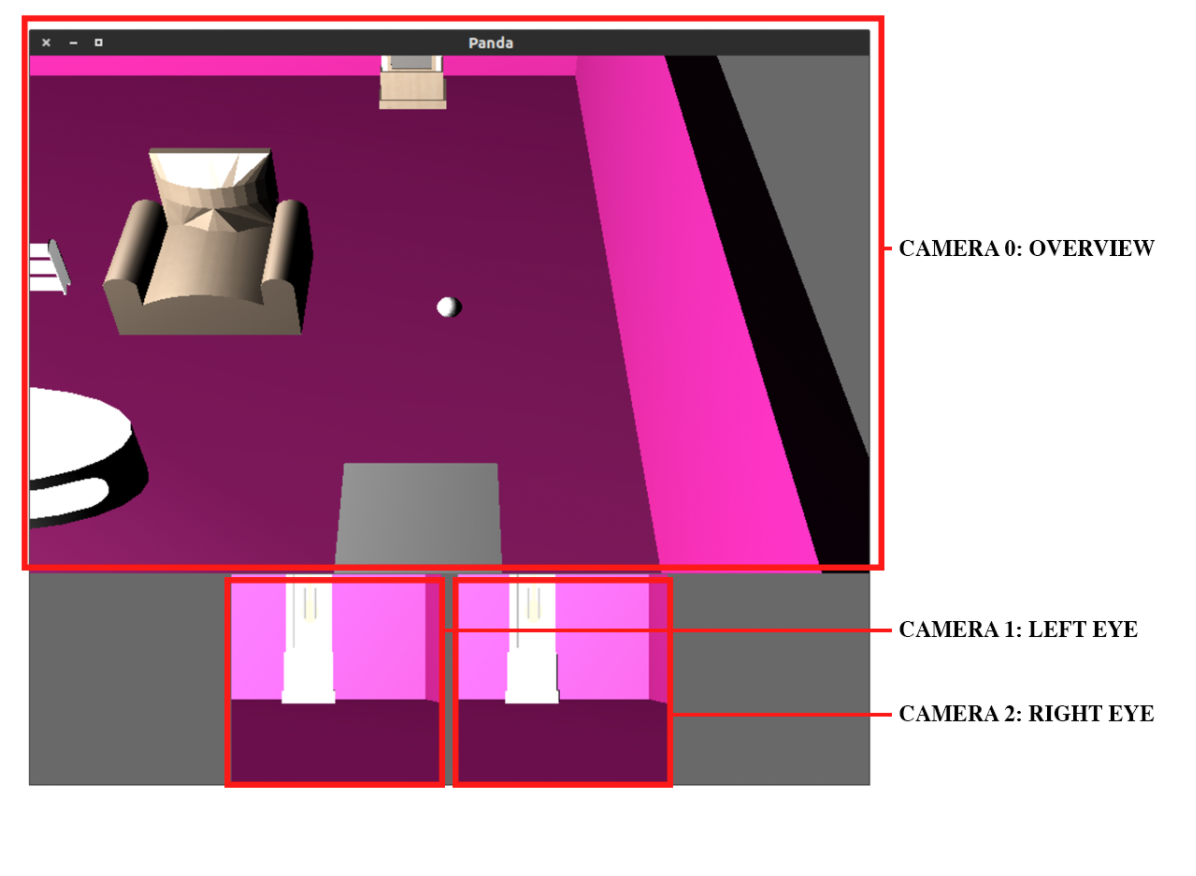
\includegraphics[width=\linewidth]{images/godview.png}
  \caption{Simulated Environment}
  \label{fig:boat1}
\end{figure}